
\documentclass[2dCFT-lecture.tex]{subfiles}

\begin{document}



\setcounter{tocdepth}{2}
%\maketitle
\section{Modular Invariant Partition Functions}

We have already seen some examples of modular invariant partition functions, such as
torus partition functions of the free boson/fermion \S\ref{sec:free-torus}, and minimal models \S\ref{sec:characters-MM}.
We first review a free boson on a circle and look into its modular invariance in special cases.
Then, we make further investigations on other possibilities.

When we consider torus partition function it should always be modular invariant because it is a consequence of the geometry, torus.
Nonetheless, it is non-trivial to see in some cases. Instead, by requiring the modular invariance gives us some useful information,
which can be seen in \S\ref{sec:orbif-part-funct}.


\subsection{Free Boson on a Circle}
\label{sec:free-boson-circle}

Let us first focus on a single free boson on a circle.
The partition function on a circle of radius $R$ is, as we have seen in \eqref{eq:bosonZ}:
\begin{equation}
\mathcal{Z}_{R}(\tau,\overline{\tau})
 = \Tr \bigg( q^{L_0 -\frac{c}{24}} \overline{q}^{\overline{L}_0-\frac{c}{24}} \bigg)
 = \frac{1}{|\eta(\tau)|^2}\sum_{n,w} q^{\frac12 (\frac{n}{R}+\frac{Rw}{2})^2} \overline{q}^{\frac12 (\frac{n}{R}-\frac{Rw}{2})^2}, \label{eq:bosonZ1}
\end{equation}
where we changed conventions, and here, $n$ is for KK-momentum and $w$ for winding number.
Note that $R$ dependence of the partition function means that the theory depends on the radius $R$.
We will see peculiar features of theories (partition functions) at specific values of the radius.
Now, let us study the partition function on a special radius $R = \sqrt{2k}$
with $k \in \mathbb{Z}^{+}$.
Rearranging the summation, the
partition function can be written as
\begin{align}
 \mathcal{Z}_{\sqrt{2k}} (\tau,\overline \tau) &= \frac{1}{\abs{\eta(\tau)}^2} \sum_{n,w \in \mathbb Z} q^{\frac{1}{4k} (n+kw)^2} \overline{q}^{\frac{1}{4k} (n-kw)^2}
 = \frac{1}{\abs{\eta(\tau)}^2} \sum_{m \in \mathbb Z_{2k} \atop n_L,n_R \in \mathbb Z} q^{\frac{1}{4k} (m+2kn_L)^2} \overline{q}^{\frac{1}{4k} (m-2kn_R)^2}  \nonumber\\
 &= \frac{1}{\abs{\eta(\tau)}^2} \sum_{m \in \mathbb Z_{2k}} \left| \Theta_{m,k} (\tau) \right|^2~,
\end{align}
where the range of $k$ is $-k+1 \le m \le k$, $\Theta$-function was defined in \eqref{Theta function}.
Conformal field theories corresponding to these
partition functions are commonly denoted as
$\widehat{\mathfrak{u}(1)}_k$, and we use this notation for the subscript from now on. Indeed, for $k = 1$, we find
\begin{equation}
\label{partition function k = 1}
  \mathcal{Z}_{\widehat{\mathfrak{u}(1)}_1}(\tau,\overline{\tau})
  = \frac{1}{\abs{\eta(\tau)}^2}
  \bigg(
  \abs{\Theta_{0,1}}^2 + \abs{\Theta_{1,1}}^2
  \bigg)
  = \chi_0^{(1)}\overline{\chi}_0^{(1)}
  +\chi_1^{(1)}\overline{\chi}_1^{(1)}
  \, ,
\end{equation}
where $\chi_j^{(1)}$ is the character of $\widehat{\mathfrak{su}(2)}_1$ as we will see below. As we have seen in \S\ref{sec:SU(2)k}, $k=1$ is actually the self-dual point, and the symmetry $\widehat{\mathfrak{u}(1)}_1$ is enhanced to $\widehat{\mathfrak{su}(2)}_1$,


From the definition of $\Theta$-function, it is easy to see
the T-transformations for $\Theta$- function, we have
\begin{equation}
  \Theta_{m,k}(\tau+1) = e^{\pi i m^2 / 2k}
  \Theta_{m,k}(\tau)\, .
\end{equation}
For the modular S-transformation, we have
\begin{equation}
 \Theta_{m,k} \bigg(
 -\frac{1}{\tau}
 \bigg)
 = \sqrt{-i \tau}
 \sum_{m' = -k + 1}^ k
 S_{m,m'}
 \Theta_{m',k}(\tau)\, ,
\end{equation}
with the modular S-matrix
\begin{equation}
 S_{m,m'} = \frac{1}{\sqrt{2k}}
 \exp(-\pi i \frac{m m'}{k})\, .
\end{equation}
For $k=1$ case, the S-transformation for the characters
in \eqref{partition function k = 1} can be
inferred from the transformation properties of the
$\Theta$- and $\eta$-functions
\begin{equation}
\chi^{(1)}_m\big(
-\frac{1}{\tau}
\big) = \sum_{m'=0}^1
S_{m,m'} \chi_{m'}^{(1)}(\tau)
\end{equation}
Following what we have done when constructing modular invariant
partition function in minimal model, we can write the partition function
\eqref{partition function k = 1} as
\begin{equation}
 \mathcal{Z}_{\widehat{\mathfrak{u}(1)}_1}(\tau,\overline{\tau}) =
 (\chi^{(1)}_0, \chi_1^{(1)})
 \mqty(1&0\\0&1)
 \mqty(\overline{\chi}_0^{(1)}\\ \overline{\chi_1}^{(1)})
 =\vec{\chi}^T M \vec{\overline{\chi}}\, ,
\end{equation}
where $M$ is the identity matrix in this case.
The S-transformation of partition function now reads
\begin{equation}
  \mathcal{Z}_{\widehat{\mathfrak{u}(1)}_1} \bigg(
  -\frac{1}{\tau},
  -\frac{1}{\overline{\tau}}
  \bigg)
  =\vec{\chi}^T S^T M S^*\vec{\overline{\chi}}\, .
\end{equation}
Since $S^T = S$ from the definition of S matrix, the
condition for invariance under modular S-transformation
for the partition function now reads
\begin{equation}
 S M S^{\dagger} = M \, .
\end{equation}
This is obviously true in this simple case. Because
under T-transformations the characters $\chi_m^{(1)}$
only acquire a phase, we have shown that
$\mathcal{Z}_{\widehat{\mathfrak{u}(1)}_1}(\tau,\overline{\tau})$ is modular invariant.
This process can be generalized to construct more
complicated modular invariant partition function.




Let us look into $k=2$ case as well. The modular invariant partition function is given as follows.
\begin{align}
 \cZ_{\widehat{u(1)}_2} = \sum_{-1 \le m \le 2} \left| \frac{\Theta_{m,2}(\tau)}{\eta(\tau)} \right|^2
 = \frac{1}{2} \left\{\left| \frac{\vartheta_2(\tau)}{\eta(\tau)} \right|^2 +\left| \frac{\vartheta_3(\tau)}{\eta(\tau)} \right|^2
 +\left| \frac{\vartheta_4(\tau)}{\eta(\tau)} \right|^2 \right\}
\end{align}
Notice that the expression above is exactly the same as the torus partition function of a free complex fermion on a circle \eqref{free-fermion-minimal-model},
though the second equality above is non-trivial.
This means that a free boson on a circle at $R=2$ is equivalent to a free complex fermion, and it is called ``Boson-Fermion correspondence''
(or bosonization, fermionization).
We have already seen the equivalence in terms of operator correspondence in the homework 4.
This is a simple example of ``duality'', which provides us a pair of theories that describe the same physics
(hence their physical quantities like multi-point function and partition function etc. agree each other).
It provides not only different physical pictures but also important mathematical formulae, which we will see in homework of this week.




\subsection{Orbifold partition function}
\label{sec:orbif-part-funct}
As we saw in a free boson on a circle case, the theory depends on a ``target space''\footnote{
Target space is a space that fields take their values. In the case of a free boson on a circle,
$\varphi$ takes a value on the circle $x \sim x +2\pi R$. Hence, the target space is the circle.}
on which the theory lives.
Especially, the boundary condition plays an important role. For the circle case it is
\begin{align}
 \varphi(z e^{2\pi i}, \overline z e^{-2\pi i}) = \varphi(z, \overline z) + 2\pi w R , \qquad w \in \mathbb Z \quad \textrm{: winding number}.
 \label{eq:bosonS1BoundaryCond}
\end{align}

Now, we want to extend our knowledge to other kinds of CFT, therefore, we consider different target spaces.
What we consider here is so called orbifold.
For a manifold $M$ and a discrete group $\Gamma$, a space defined by a quotient $M/\Gamma$ with an equivalence relation
\begin{align}
 x \sim g x \qquad g \in \Gamma , \quad x \in M ,
\end{align}
could be singular, and it is, in general, called orbifold.


We consider, as the simplest example, the $\mathbb{Z}_2$-orbifold of a circle with radius $R$ \cite[ISZ88-No.40]{Yang:1987mf}.
In this case $M = S^1$ and $\Gamma = \mathbb Z_2$ whose elements are $g = \{1,-1\}$.
The non-trivial equivalence relation is, therefore, $x \sim -x$.
Resultant orbifold is denoted by $S^1/\mathbb Z_2$ (see Fig.~\ref{fig:orbifold}).
\begin{figure}[ht]
 \centering
 \begin{tikzpicture}[scale=1]
  \draw[thick] (0,0) circle[radius=1];
  \draw (0,1) node{$\times$} ;
  \draw (0,1.5) node{$x=0$} ;
  \draw (0,-1) node{$\times$} ;
  \draw (0,-1.5) node{$x=\pi R$} ;
  \draw[Stealth-Stealth,blue] (-0.7,0.6) -- (0.7,0.6) ;
  \draw[Stealth-Stealth,blue] (-0.9,0.2) -- (0.9,0.2) ;
  \draw[Stealth-Stealth,blue] (-0.9,-0.2) -- (0.9,-0.2) ;
  \draw[Stealth-Stealth,blue] (-0.7,-0.6) -- (0.7,-0.6) ;
  \draw (-2.5,0) node[blue]{Identify} ;
  \draw[-Triangle] (2,0) -- (3,0) ;
  \draw[thick] (4,-1) node{$\times$} -- (4,1) node{$\times$} ;
 \end{tikzpicture}
 \caption{From a circle ($S^1$) with radius $2\pi R$ to a $\mathbb Z_2$-orbifold ($S^1/\mathbb Z_2$) of the circle.
 We identify points $x$ and $-x$ in the circle, which leads to a finite line. There are two singular points, which are illustrated by crosses in the figure.}
 \label{fig:orbifold}
\end{figure}
Our goal is to calculate a partition function of a free boson on the orbifold.
In order to achieve this we consider a free boson on a circle $\varphi\sim \varphi + 2\pi R$,
and define a $\mathbb{Z}_2$ symmetry (orbifold) operator $\mathcal{R}$:
\begin{equation}
 \mathcal{R}: \varphi(z,\overline{z})\mapsto -\varphi(z,\overline{z})\, , \qquad \mathcal R^2 = \mathrm{Id} \, .
\end{equation}
We calculate a partition function with states
invariant under the orbifold action.
Namely, we
insert an orbifold projection operator $\frac{1}{2}(1+\mathcal{R})$ into the trace in (\ref{eq:bosonZ1}),
and the partition function reads
\begin{align}
\mathcal{Z}_{\textrm{orb}}(\tau,\overline{\tau}) &= \Tr
\bigg(
\frac{1+\mathcal{R}}{2} q^{L_0 -\frac{c}{24}}
\overline{q}^{\overline{L}_0-\frac{c}{24}}
\bigg)\notag\\
& =
\frac{1}{2}\mathcal{Z}_{R}(\tau,\overline{\tau})
+\frac{1}{2}\Tr\big(
\mathcal{R} q^{L_0-\frac{c}{24}}
\overline{q}^{\overline{L}_0-\frac{c}{24}}
\big)\, .
\end{align}
The first term contains the partition function of a
free boson on a circle which we already computed in
\eqref{eq:bosonZ1}.
Let us focus on the second term.


The action of $\mathcal{R}$ on the Laurent modes $a_n$
of $ i\partial\varphi(z)$ can be found
\def\mR{\mathcal{R}}
\begin{equation}
  \mathcal{R}a_n\mathcal{R}= -a_n \, .
\end{equation}
Hence
\begin{align}
\mathcal{R}\ket{n_1,n_2,n_3,\dots} & =
(\mR a_{-1}\mR)^{n_1}
(\mR a_{-2}\mR)^{n_2}
\dots
\mR \ket{\Omega}\notag \\
& = (-1)^{n_1+n_2+n_3 + \dots}
\ket{n_1, n_2, n_3,\dots}\, .
\end{align}
where $\ket{\Omega}$ is a ground state, and we assumed that it is invariant under $\mR$, i.e $\mR\ket{\Omega} = \ket{\Omega}$.
% we have chosen the action of $\mathcal{R}$ such
% that $\ket{0}$ is left invariant.
Now, we consider the action $\mathcal R$ on the ground states in details. Remember that the ground state is
characterized by KK-momentum and winding number, $\ket{\Omega} = |n,w \rangle$.
Since the zero mode operator $a_0$ gives eigenvalues of the states
\begin{align}
 a_0 \ket{n,w} = \left( \frac{n}{R} +\frac{Rw}{2} \right) \ket{n,w} ,
\end{align}
we see that
\begin{align}
 &a_0 \mathcal{R}\ket{n,w}
 =\mathcal{R}(\mR a_0 \mR)\ket{n,w}
 =\mathcal{R}(-a_0) \ket{n,w}
 =-\bigg(
 \frac{n}{R} + \frac{R w}{2}
  \bigg)
 \mR \ket{n,w}\, ,  \nonumber\\
 &\therefore\quad \mR \ket{m,n} \propto \ket{-m,-n}\, .
\end{align}
Therefore, only states with $\ket{m=0, n= 0}$ will
contribute in the calculation of the partition function.
Then following the same steps in \eqref{free-boson-process},
we replace the result of the free boson as
\begin{equation}
q^{-\frac{1}{24}}\prod_{n=1}^\infty\frac{1}{1-q^n}
\quad \to \quad
q^{-\frac{1}{24}}\prod_{n=1}^\infty\frac{1}{1-(-q^n)}
= \sqrt{2}\sqrt{\frac{\eta{(\tau)}}{\vartheta_2(\tau)}}\, .
\end{equation}
We thus write the partition function as
\begin{equation}
\label{Orbifold-partition-function-1}
\mathcal{Z}(\tau,\overline{\tau}) = \frac{1}{2}
\mathcal{Z}_R(\tau,\overline{\tau}) +
\abs{\frac{\eta(\tau)}{\vartheta_2(\tau)}}\, .
\end{equation}

Notice that the result \eqref{Orbifold-partition-function-1}
can not be the correct partition function because the second term is not invariant under modular transformation.
% Notice that we can realize this partition function is something wrong, thanks to modular property argument.
Recalling the free fermions partition function result, $\vartheta$-functions
enjoy the modular transformations illustrated in Fig.\ref{fig:modular-theta}.
In order for a free boson on the orbifold to have modular invariance
we are required to add so-called twisted sector, whose contributions should be
\begin{equation}
  \mathcal{Z}_{\text{tw}} (\tau,\overline{\tau}) =
  \abs{\frac{\eta(\tau)}{\vartheta_4(\tau)}}
  +
  \abs{\frac{\eta(\tau)}{\vartheta_3(\tau)}}\, .
\end{equation}
Then, the modular invariant partition function of a free boson on the
$\mathrm{Z}_2$-orbifold reads
\begin{equation}
\mathcal{Z}_{\text{orb}}(\tau,\overline{\tau})=
\frac{1}{2}
\mathcal{Z}_R(\tau,\overline{\tau}) +
\abs{\frac{\eta(\tau)}{\vartheta_2(\tau)}}
+
\abs{\frac{\eta(\tau)}{\vartheta_4(\tau)}}
+
\abs{\frac{\eta(\tau)}{\vartheta_3(\tau)}}\, .
\label{eq:orbfioldPF}
\end{equation}
Although we derived the correct result by requiring modular invariance here,
it is instructive to see what is the physical realization of the twisted sector.

\subsubsection*{Twisted sector}

Recall that when we calculate torus partition function of a free fermion on a circle,
we considered Neveu-Schwarz (NS) sector as well as Ramond (R) sector, which are realized as follows.
\begin{align}
 &\psi\left( e^{2\pi i} z \right) = \psi(z) \qquad\!\quad \textrm{NS} , \\
 &\psi\left( e^{2\pi i} z \right) = -\psi(z) \qquad \textrm{R} ,
\end{align}
where only the holomorphic parts are shown.
We realize that the NS sector corresponds to
the boundary condition of a free boson (\ref{eq:bosonS1BoundaryCond}),
and wonder if there is R sector like boundary condition.
There, indeed, exists due to the operation $\mR$:
\begin{align}
 \varphi(z e^{2\pi i}, \overline z e^{-2\pi i}) = \mR \varphi(z, \overline z) + 2\pi w R = -\varphi(z, \overline z) + 2\pi w R .
\end{align}
In order to realize this boundary condition the mode have to become ``half-integers'' modes:
\begin{align}
 &\varphi(z,\overline z) = \varphi(z) +\overline\varphi(\overline z) , \nonumber\\
 &\quad\varphi(z) = \frac{x}{2} +i \sum_{n \in \mathbb Z +\frac{1}{2}} \frac{1}{n} \frac{a_n}{z^n} .
\end{align}
There are two possible value for the zero mode $x$; one is $x=0 \ (w=0)$ and the other is $x = \pi R \ (w=1)$.
Due to the shift of the modes the zero point energy is also modified as follows (recall homework 5: $\zeta$-function regularization).
\begin{align}
 \frac{1}{2} \sum_{n=0}^\infty n = -\frac{1}{24} \quad \to \quad
 \frac{1}{2} \sum_{n=0}^\infty (n+\frac{1}{2}) = -\frac{1}{24} +\frac{1}{16} = \frac{1}{48} .
\end{align}
Therefore, we have following contribution:
\begin{align}
 &\frac{1}{2} \Tr_\mathrm{tw} \left[ q^{L_0 -\frac{1}{24}} \overline q^{\overline{L_0} -\frac{1}{24}} \right] \quad \textrm{with} \quad
 L_0 = \sum_{n=1}^\infty a_{-n+\frac{1}{2}} a_{n-\frac{1}{2}} +\frac{1}{16} \nonumber\\
 &= \frac{1}{2}\cdot 2 \cdot |q|^{2\cdot \frac{1}{48}} \prod_{n=1}^\infty \left| \frac{1}{1-q^{n-\frac{1}{2}}} \right|^2
 = \left| \frac{\eta(\tau)}{\vartheta_4(\tau)} \right| ,
\end{align}
where the factor of two in the coefficient is coming from the two contributions of zero modes $x=0$ and $x=\pi R$.
Similarly,
\begin{align}
 &\frac{1}{2} \Tr_\mathrm{tw} \left[ \mathcal R q^{L_0 -\frac{1}{24}} \overline q^{\overline{L_0} -\frac{1}{24}} \right] \quad \textrm{with} \quad
 L_0 = \sum_{n=1}^\infty a_{-n+\frac{1}{2}} a_{n-\frac{1}{2}} +\frac{1}{16} \nonumber\\
 &= |q|^{\frac{1}{24}} \prod_{n=1}^\infty \left| \frac{1}{1+q^{n-\frac{1}{2}}} \right|^2
 = \left| \frac{\eta(\tau)}{\vartheta_3(\tau)} \right| .
\end{align}
As we expected we have correct contributions from the twisted sector.
There are several comments:
\begin{itemize}
 \item $\cZ_\mathrm{orb}$ depends on radius $R$ only through $\cZ_R$, and hence, it enjoys T-duality:
       $\cZ_\mathrm{orb}(R) = Z_\mathrm{orb}(2/R)$.
 \item One can see that $\cZ_\mathrm{orb}(R=\sqrt 2) =\cZ_R (R = 2\sqrt 2)$.
       Namely, a free boson on a circle with $R=\sqrt 2$ is equivalent to that on an $S^1/\mathbb Z_2$ with $R=2\sqrt 2$.
       As we stressed before, theories depend on their radii, and two branches of a free boson theory
       intersect at the point of moduli space of the theory (see Fig.~\ref{fig:moduliOfPF}).
      \item  The $\cN=2$ superconformal symmetry arises at $R_{\textrm{circ}}=\sqrt{3}$, and  $\cN=1$ superconformal symmetry arises at $R_{\textrm{orb}}=\sqrt{3}$ \cite[ISZ88-No.39]{Friedan:1989yz} \cite{Yang:1987bj}.
       \item  In fact, a CFT with $c=1$ can be constructed by taking a quotient of the $\SU(2)_1$ current algebra by its finite subgroup. There is one-to-one correspondence between the finite subgroups of $\SU(2)$ and the ADE Dynkin diagrams, which is called the \textbf{McKay correspondence}. The CFTs corresponding to $T$ $(E_6)$, $O$ $(E_7)$, and $I$ $(E_8)$ are isolated (does not allow deformation) \cite[ISZ88-No.33]{Pasquier:1986jc} \cite[ISZ88-No.41]{Ginsparg:1987eb}.
\begin{figure}[ht]
 \centering
 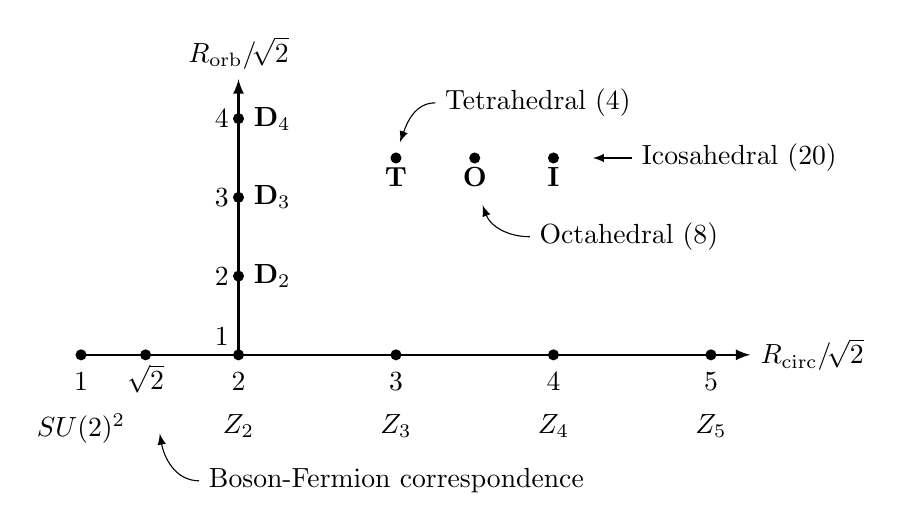
\begin{tikzpicture}
  \draw [-latex,thick] (0,0) -- (8.5,0) node[right]{$R_\mathrm{circ}/\!\sqrt{2}$} ;
  \draw [-latex,thick] (2,0) -- (2,3.5) node[above]{$R_\mathrm{orb}/\!\sqrt{2}$};
  \fill (0,0) circle (2pt) node[below=3pt]{1} node[below=18pt]{$SU(2)^2$};
  \fill (0.82,0) circle (2pt)  node[below]{$\sqrt 2$} ;
  \draw [latex-, out=-80, in=180] (1,-1) to (1.5,-1.6) node[right]{Boson-Fermion correspondence} ;
  \fill (2,0) circle (2pt) node[below=3pt]{2} node[above left]{1} node[below=18pt]{$\mathbb Z_2$} ;
  \fill (4,0) circle (2pt) node[below=3pt]{3} node[below=18pt]{$\mathbb Z_3$} ;
  \fill (6,0) circle (2pt) node[below=3pt]{4} node[below=18pt]{$\mathbb Z_4$} ;
  \fill (8,0) circle (2pt) node[below=3pt]{5} node[below=18pt]{$\mathbb Z_5$} ;
  \fill (2,1) circle (2pt) node[left]{2} node[right=2pt]{$\mathbf{D}_2$} ;
  \fill (2,2) circle (2pt) node[left]{3} node[right=2pt]{$\mathbf{D}_3$} ;
  \fill (2,3) circle (2pt) node[left]{4} node[right=2pt]{$\mathbf{D}_4$} ;
  \fill (4,2.5) circle (2pt) node[below]{\textbf T} ;
  \draw [latex-, out=70, in=180] (4.05,2.7) to (4.5,3.2) node[right]{Tetrahedral (4)} ;
  \fill (5,2.5) circle (2pt) node[below]{\textbf O} ;
  \draw [latex-, out=-70, in=180] (5.1,1.9) to (5.7,1.5) node[right]{Octahedral (8)} ;
  \fill (6,2.5) circle (2pt) node[below]{\textbf I} ;
  \draw [latex-] (6.5,2.5) to (7,2.5) node[right]{Icosahedral (20)} ;
 \end{tikzpicture}
 \caption{Moduli space of 2d CFTs with $c=1$. The horizontal allow expresses so called toroidal branch, and the vertical allow does orbifold branch.
 $R_\mathrm{circ}$ is radius of a circle and $R_\mathrm{orb}$ is that of the orbifold.
 $SU(2)^2$ is the symmetry that the theory has at the self-dual point. $\mathbb Z_k$, $\mathbf D_k$, $T$, $O$, and $I$ are
 the subgroup of the $SU(2)^2$ at corresponding points illustrated above.. For more details see \cite[ISZ88-No.41]{Ginsparg:1987eb}.}
 \label{fig:moduliOfPF}
\end{figure}
\end{itemize}


So far, only a specific orbifold example are illustrated.
For general orbifold $\Gamma$ we can do parallel computations as follows.
Let us consider a field in a cylinder coordinates $\Phi(\sigma,\tau)$, and for $g, h \in \Gamma$, we have
\begin{align}
 \Phi(\sigma,\tau+2\pi) = g \cdot \Phi(\sigma,\tau) , \nonumber\\
 \Phi(\sigma+2\pi,\tau) = h \cdot \Phi(\sigma,\tau) .
\end{align}
Note that $\sigma$ and $\tau$ are commutative on torus, hence, $g$ and $h$ should also be commutative, i.e $gh=hg$.
As we have seen before, time-like orbifold condition (the first line above) is realized by operator insertions,
and the space-like orbifold condition (the second line above) is realized by twisted sectors (trace over twisted Hilbert space):
\begin{align}
 \cZ_{(g,h)} (\tau,\overline \tau) = \Tr_{\mathcal H_h} \left[ g q^{L_0 -\frac{c}{24}} \overline q^{\overline{L_0} -\frac{c}{24}} \right] ,
\end{align}
and the full partition function is given by sum over all possible values of $g$ and $h$:
\begin{align}
 \cZ_{M/\Gamma} (\tau,\overline \tau) = \frac{1}{|\Gamma|} \sum_{g,h \in \Gamma \atop gh = hg} \cZ_{(g,h)} (\tau,\overline \tau) ,
\end{align}
where $|\Gamma|$ is the degree of a discrete group $\Gamma$.
One should check that this formula reproduces our result of $S^1/\mathbb Z_2$.



\subsection{$\widehat{\mathfrak{su}(2)}_k$ characters}\label{sec:su2k-character}
It has been briefly mentioned in \S\ref{sec:free-boson-circle} that $\widehat{\mathfrak{u}(1)}_1$ theory has actually $\widehat{\mathfrak{su}(2)}_1$ symmetry,
therefore, its partition function can be expressed by so called $\widehat{\mathfrak{su}(2)}_1$ character.
Here, we derive the $\widehat{\mathfrak{su}(2)}_1$ character by considering a free boson on a circle with $R = \sqrt 2$.


Recall that the theory can be characterized by three operators (for more details see \S\ref{sec:SU(2)k}):
\begin{align}
 J(z) = \frac{i\partial\varphi (z)}{\sqrt 2} , \qquad J^\pm (z) = :\! e^{\pm i \sqrt 2 \varphi(z)} \!: .
\end{align}
OPE calculation leads to following commutation relations
\begin{align}
 &[J^3_n,J^\pm_m] = \pm J^\pm_{n+m}, \nonumber\\
 &[J^+_n,J^-_m] = 2 J^3_{n+m} +n\delta_{n+m,0}, \nonumber\\
 &[L_0,J^a_n] = -n J^a_{n} \qquad (a=3,\pm) .
\end{align}
Let us consider the highest weight representation of the theory.
Notice that $L_0$ and $J^3_0$ commutes, hence, the highest weight vector(states) should be characterized by their eigenvalues $h$ and $j$,
and the vector is defined as follows.
\begin{align}
 &J^\pm_n \ket{h,j} = J^3_n \ket{h,j} = 0 \qquad (n \ge 1) ,  \nonumber\\
 &J^+_0 \ket{h,j} = \left(J^-_0\right)^{2j+1} \ket{h,j} = 0 ,  \nonumber\\
 &J^3_0 \ket{h,j} = j \ket{h,j} .
\end{align}
Note that from the argument of \S\ref{sec:SU(2)k} $j$ can only be $j=0,\frac12$ for $k=1$.
For $j=0$, the corresponding conformal dimension is $h=0$, and for $j=\frac{1}{2}$, that is $h=\frac{1}{4}$.
Basically, we can construct an integrable representation by acting the following operators to the highest weight vectors:
\begin{align}
 J^-_n \quad (n\le 0) , \qquad J^3_m, \ J^+_m \quad (m < 0).
\end{align}
We organize these creation operators in a following manner.
\begin{align}
 J^+_{(n)} = J^+_{-n} , \qquad
 J^-_{(n)} = J^-_{+n} , \qquad
 J^3_{(n)} = J^3_{0} -\frac{n}{2} .
\end{align}
Notice that each $J^a_{(n)}$ forms $\mathfrak{su}(2)$ algebra (call them $\mathfrak{su}(2)_{(n)}$).

Let us consider one $\ket{0,0}$ of the highest vectors.
Since $J^3_{(0)} \ket{0,0} = 0$ the vector is singlet under the $\mathfrak{su}(2)_{(0)}$.
On the other hand, $J^3_{(1)} \ket{0,0} = -\frac{1}{2} \ket{0,0}$, $J^-_{(1)} \ket{0,0} = 0$, and hence,
it should be a spin-$\frac{1}{2}$ representation of $\mathfrak{su}(2)_{(1)}$.
Therefore, there is exactly one other states $J^+_{(1)} \ket{0,0}$.
Repeating similar procedures for $J^+_{(1)} \ket{0,0}$, and it turns that
$J^+_{(1)} \ket{0,0}$ is singlet under $\mathfrak{su}(2)_{(2)}$ but doublet under $\mathfrak{su}(2)_{(3)}$.
In summary, we have a tower of $J^+_{(n)}$ for odd $n$ (let us set $n=2p-1$):
\begin{align}
 &J^+_{(1)} J^+_{(3)} J^+_{(5)} \cdots J^+_{(2p-1)} \ket{0,0} := \ket{p; 0,0} ,  \nonumber\\
 &L_0 \ket{p; 0,0} = \sum_{m=1}^{p} (2m-1) \ket{p; 0,0} = p^2 \ket{p; 0,0} ,  \nonumber\\
 &J^3_0 \ket{p; 0,0} = p \ket{p; 0,0} .
\end{align}
We can also consider negative $n=-2p+1$ ($p \in \mathbb Z_{\ge 1}$), and the resultant tower is
\begin{align}
 &J^-_{(-1)} J^-_{(-3)} J^-_{(-5)} \cdots J^-_{(-2p+1)} \ket{0,0} := \ket{-p; 0,0} ,  \nonumber\\
 &L_0 \ket{-p; 0,0} = \sum_{m=1}^{p} (2m-1) \ket{-p; 0,0} = p^2 \ket{-p; 0,0} ,  \nonumber\\
 &J^3_0 \ket{-p; 0,0} = -p \ket{-p; 0,0} .
\end{align}
Notice that these tower corresponds to vertex operators:
\begin{align}
 \ket{p; 0,0} \quad &\leftrightarrow \quad :\! e^{+ i p \sqrt 2 \varphi(z)} \!:  , \nonumber\\
 \ket{-p; 0,0} \quad &\leftrightarrow \quad :\! e^{- i p \sqrt 2 \varphi(z)} \!:  , \nonumber\\
 \ket{0; 0,0} := \ket{0,0} \quad &\leftrightarrow \quad 1  .
\end{align}


\begin{figure}[ht]
 \centering
 \begin{tikzpicture}
 \begin{scope}
  \draw[step=1,very thin, lightgray] (-3,0) grid (3,9) ;
  \draw [-latex] (-3.5,0) -- (3.5,0) node[right]{$J^3_0$} ;
  \draw [-latex] (0,0) -- (0,9.5) node[above]{$L_0$};
  \fill (0,0) circle (2pt) node[below=3pt]{0} ;
  \fill (1,1) circle (2pt) (2,4) circle (2pt) (3,9) circle (2pt) (-1,1) circle (2pt) ;
  \draw[-Stealth, thick] (0,0) -- (1,1) ;
  \draw (1.1,0.4) node{$J^+_{(1)}$} ;
  \draw[-Stealth, thick] (1,1) -- (2,4) ;
  \draw (2,2.2) node{$J^+_{(3)}$} ;
  \draw[-Stealth, thick] (2,4) -- (3,9) ;
  \draw (3,6.2) node{$J^+_{(5)}$} ;
  \draw[-Stealth, thick] (0,0) -- (-1,1) ;
  \draw (-1.1,0.4) node{$J^-_{(-1)}$} ;
  \fill (-2.7,1.5) circle (2pt) (-2.7,3) circle (2pt) (-2.7,5.5) circle (2pt) ;
  \draw[-Stealth, thick] (-2.7,1.5) -- (-2.7,2.5) ;
  \draw (-2,1.9) node{$J^3_{(-1)}$} ;
  \draw[-Stealth, thick] (-2.7,3) -- (-2.7,5) ;
  \draw (-1.8,4) node{$J^3_{(-2)}, \atop \left(J^3_{(-1)}\right)^2$} ;
  \draw[-Stealth, thick] (-2.7,5.5) -- (-2.7,8.5) ;
  \draw (-1.3,7) node{$J^3_{(-3)},\ \left(J^3_{(-1)}\right)^3, \atop J^3_{(-2)} J^3_{(-1)} $} ;
  \draw [latex-, out=120, in=180] (-2.9,7) to (-2.7,9) node[right]{For each dot} ;
  \draw [latex-, out=120, in=180] (-2.9,4) to (-2.7,9) ;
  \draw [latex-, out=120, in=180] (-2.9,2.2) to (-2.7,9) ;
  \draw (1,0) node[below=3pt]{1};
  \draw (2,0) node[below=3pt]{2};
  \draw (3,0) node[below=3pt]{3};
  \draw (-1,0) node[below=3pt]{$-1$};
  \draw (-2,0) node[below=3pt]{$-2$};
  \draw (-3,0) node[below=3pt]{$-3$};
  \draw (0,-1.3) node{$j=0$} ;
 \end{scope}
 \begin{scope}[shift={(8,0)}]
  \draw[step=1,very thin, lightgray] (-3,0) grid (3,9) ;
  \draw [-latex] (-3.5,0) -- (3.5,0) node[right]{$J^3_0$} ;
  \draw [-latex] (0,0) -- (0,9.5) node[above]{$L_0$};
  % \fill (0,0) circle (2pt) node[below=3pt]{0} ;
  % \fill (1,1) circle (2pt) (2,4) circle (2pt) (3,9) circle (2pt) (-1,1) circle (2pt) ;
  % \draw[-Stealth, thick] (0,0) -- (1,1) ;
  % \draw (1.1,0.4) node{$J^+_{(1)}$} ;
  % \draw[-Stealth, thick] (1,1) -- (2,4) ;
  % \draw (2,2.2) node{$J^+_{(3)}$} ;
  % \draw[-Stealth, thick] (2,4) -- (3,9) ;
  % \draw (3,6.2) node{$J^+_{(5)}$} ;
  % \draw[-Stealth, thick] (0,0) -- (-1,1) ;
  % \draw (-1.1,0.4) node{$J^-_{(-1)}$} ;
  \fill (-1.5,9/4) circle (2pt) (0.5,1/4) circle (2pt) (1.5,9/4) circle (2pt) (2.5,25/4) circle (2pt) (-0.5,1/4) circle (2pt) ;
  \draw[Stealth-, thick] (-1/2,1/4) -- (1/2,1/4) ;
  \draw (-0.3,0.75) node{$J^-_{(0)}$} ;
  \draw[-Stealth, thick] (-1/2,1/4) -- (-3/2,9/4) ;
  \draw (-1.6,1.1) node{$J^-_{(-2)}$} ;
  \draw[-Stealth, thick] (1/2,1/4) -- (3/2,9/4) ;
  \draw (1.6,1.1) node{$J^+_{(2)}$} ;
  \draw[-Stealth, thick] (3/2,9/4) -- (5/2,25/4) ;
  \draw (2.6,4.1) node{$J^+_{(4)}$} ;
  \draw[thick] (5/2,25/4) -- (3,37/4) ;
  \draw (0,0) node[below=3pt]{0};
  \draw (1,0) node[below=3pt]{1};
  \draw (2,0) node[below=3pt]{2};
  \draw (3,0) node[below=3pt]{3};
  \draw (-1,0) node[below=3pt]{$-1$};
  \draw (-2,0) node[below=3pt]{$-2$};
  \draw (-3,0) node[below=3pt]{$-3$};
  \draw (0,-1.3) node{$j=\frac{1}{2}$} ;
 \end{scope}
 \end{tikzpicture}
 \caption{Highest weight representation of $\widehat{\mathfrak{su}(2)}_{1}$.
 For each dot there must be degenerate vertical arrows with integer length, which express descendant fields.}
 \label{fig:su2_1states}
\end{figure}


The other highest weight vector $\ket{\frac{1}{4},\frac{1}{2}}$ is doublet under $\mathfrak{su}(2)_{(0)}$.
$\ket{\frac{1}{4},\frac{1}{2}}$ is singlet under $\mathfrak{su}(2)_{(1)}$ and doublet under $\mathfrak{su}(2)_{(2)}$. On the other hand, $J^-_{(0)} \ket{\frac{1}{4},\frac{1}{2}}$ is singlet under $\mathfrak{su}(2)_{(-1)}$ and doublet under $\mathfrak{su}(2)_{(-2)}$.
Therefore, similar tower for $\ket{\frac{1}{4},\frac{1}{2}}$ is ($n=2q \ge 2$)
\begin{align}
 &J^+_{(2)} J^+_{(4)} \cdots J^+_{(2q)} \ket{\frac{1}{4},\frac{1}{2}} := \ket{q; \frac{1}{4},\frac{1}{2}} ,  \nonumber\\
 &L_0 \ket{q; \frac{1}{4},\frac{1}{2}} = \left(\frac{1}{4} +\sum_{m=1}^{q} 2m \right) \ket{q; \frac{1}{4},\frac{1}{2}}
 = \left(q+\frac{1}{2}\right)^2 \ket{q; \frac{1}{4},\frac{1}{2}} ,  \nonumber\\
 &J^3_0 \ket{q; \frac{1}{4},\frac{1}{2}} = \left(q+\frac{1}{2} \right) \ket{p; 0,0} ,
\end{align}
and for $J^-_{(0)} \ket{\frac{1}{4},\frac{1}{2}}$ ($n=-2q \le 0$)
\begin{align}
 &J^-_{(0)}  J^-_{(-2)} J^-_{(-4)} \cdots J^-_{(-2q)} \ket{\frac{1}{4},\frac{1}{2}} := \ket{-q; \frac{1}{4},\frac{1}{2}} ,  \nonumber\\
 &L_0 \ket{-q; \frac{1}{4},\frac{1}{2}} = \left(\frac{1}{4} +\sum_{m=1}^{q} 2m \right) \ket{q; \frac{1}{4},\frac{1}{2}}
 = \left(q+\frac{1}{2}\right)^2 \ket{q; \frac{1}{4},\frac{1}{2}} ,  \nonumber\\
 &J^3_0 \ket{q; \frac{1}{4},\frac{1}{2}} = -\left(q+\frac{1}{2} \right) \ket{p; 0,0} .
\end{align}
Again, we can see corresponding vertex operators
\begin{align}
 \ket{q; \frac14,\frac12} \quad &\leftrightarrow \quad :\! e^{+ i \frac{2q-1}{\sqrt 2} \varphi(z)} \!:  , \nonumber\\
 \ket{-q;\frac14,\frac12} \quad &\leftrightarrow \quad :\! e^{- i \frac{2q+1}{\sqrt 2} \varphi(z)} \!:  .
\end{align}
Recall that we still have $J^3_{-n}\ (n\ge 1) \sim \varphi^{(n)} = \frac{\partial^n}{\partial z^n} \varphi(z)$,
which can freely act on each tower.
Consequently,  the character of the spin-$j$ highest weight representation of $\widehat{\mathfrak{su}(2)}_{1}$
\begin{align}
 \chi_{2j}^{(1)} (\tau,z) = \Tr_{j} \left[ q^{L_0 -\frac{1}{24}} y^{J^3_0} \right] , \quad (y=e^{2\pi i z})
\end{align}
can be read off
\begin{align}
 &\chi_{0}^{(1)} (\tau,z) = \frac{\Theta_{0,1}(\tau,z)}{\eta(\tau)} ,  \nonumber\\
 &\chi_{1}^{(1)} (\tau,z) = \frac{\Theta_{1,1}(\tau,z)}{\eta(\tau)} ,   \nonumber
\end{align}
where
$$\Theta_{l,k}(\tau,z) := \sum_{n\in\mathbb{Z}+\frac{l}{2k}}
 q^{k n^2}y^{k n}$$
 reduce to the one
introduced in \eqref{Theta function} at $z=0$.
It is now obvious that the $\eta$-function is coming from the action of $\varphi^{(n)}$ ($n\ge 1$)
and the rest is from $:\! e^{i n\sqrt 2 \varphi(z)} \!:$ ($n \in \mathbb Z +j$).
See Fig.~\ref{fig:su2_1states} for the summary.



In general, irreducible representations of $\widehat{\mathfrak{su}(2)}_k$  require more careful treatment. Given a  highest weight state $|h,j\rangle$ in \eqref{HWS-su2},  one can obtain the Verma module $V(h,j)$ by acting $J_0^-$ and $J_n^a$ for $n<0$. However, like the Virasoro modules considered in \S\ref{sec:MM}, the Verma module is generally not irreducible  because it contains null states $|\chi\rangle$ which satisfy
$$
 J_{0}^{+}  |\chi \rangle=0 ,\qquad  J_{n}^{a}  |\chi \rangle=0 , \quad n > 0 , \quad a=0 , \pm ~.
$$
The Verma module $J(h,j)$ generated by the null states $|\chi\rangle$ become a (maximal proper) submodule of $V(h,j)$. Subsequently,  the quotient module
$$L(h,j):=V(h,j)/J(h,j)$$
becomes irreducible, which is called the \textbf{integrable representation} of highest weight $|h,j\rangle$. For a general affine Lie algebra $\wh \frakg_k$, one can construct an irreducible module in a similar fashion and its character is called the \textbf{Weyl-Kac character formula}. By refering the reader to \cite[\S14.4]{francesco2012conformal} for the derivation, we just write the Weyl-Kac character formula of the integrable representation of highest weight $|h,\frac l2\rangle$ for  $\widehat{\mathfrak{su}(2)}_k$  for $0\leq l\leq k$
\begin{equation}
\label{su2k-character}
\chi_l^{(k)} (\tau,z)
= \frac{\Theta_{l+1,k+2}(\tau,z) - \Theta_{-l-1,k+2}(\tau,z)}
{\Theta_{1,2}(\tau,z)-\Theta_{-1,2}(\tau,z)}\, .
\end{equation}
We can calculate the modular $S$-matrix for the character
\eqref{su2k-character} as
\begin{equation}
\label{S-matrix character}
 S^{(k)}_{l l'} =
 \sqrt{\frac{2}{k+2}}
 \sin \bigg(
 \frac{\pi}{k+2}
 (l+1)(l'+1)
 \bigg)
 \qquad
 \text{with}\quad
 l,l' = 0, \dots , k\, .
\end{equation}


We now want to construct modular invariant partition
functions out of the characters \eqref{su2k-character}.
This amounts to determining all matrices
$M_{ll'}$ such that
\begin{equation}
\label{su2k-partition function}
 \mathcal{Z}_{\widehat{\mathfrak{su}(2)}_k}(\tau,\overline{\tau}) =
 \sum_{l,l'}
 \chi_l^{(k)}(\tau)
 M^{(k)}_{ll'}
 \overline{\chi_{l'}}^{(k)}(\overline{\tau})\, .
\end{equation}
is modular invariant. The invariance under the $S$-transformation
requires
\begin{equation}
 S^{(k)T} M^{(k)} S^{(k)*} = M^{(k)}\, .
\end{equation}
$S^{(k)}$ in \eqref{S-matrix character} is symmetric
and real, thus we find the condition
\begin{equation}
 \comm{M^{(k)}}{S^{(k)}} = 0\, .
\end{equation}
We have already encountered this relation in minimal
model modular invariant formula \eqref{relation N S}.
There are further constraints for entries $M^{(k)}_{ll'}$.
Since $M^{(k)}_{ll'}$ have the interpretation
as the number of degeneracies of states in the Hilbert space,
they must be non-negative integers.
In addition, for the vacuum to only appear once, we have to
require $M^{(k)}_{00}=1$.
Furthermore, it turns out that in order for \eqref{su2k-partition function} to be invariant under
$T$-transformations, one has to satisfy the level-matching
condition $h_l - \overline{h}_{l'}\in \mathbb{Z}$.

\begin{table}[htbp]
	\centering
	\begin{tabular}{lll}
		\toprule
		Level
		& Partition function ($\mathcal{Z}_{\widehat{\mathfrak{su}(2)}_k}$)
		& Type
		\\
		\midrule
		$k=n$
		&
		$ \sum_{l=0}^{n}\abs{\chi_l}^2$
		& $A_{n+1}\, , \, n\geq 1 $
		\\
		&&\\
		$k = 4n$
		&
		$\sum_{l=0}^{n-1}
		\abs{\chi_{2l} + \chi_{k-2l}}^2
		+2|\chi_{\frac{k}{2}}|^2
		$
		& $
		D_{2n+2}\, , \, n\geq 1
		$
		\\
		&&\\
		$k=4n-2$
		& $
		 \sum_{l=0}^{k/2}
		|\chi_{2l}|^2
		+ \sum_{l=0}^{2n-2}
		\chi_{2l+1}\overline{\chi}_{k-2l-1}
		$
		& $
		D_{2n+1}\, , \, n\geq 2
		$
		\\
		&&\\
		$k=10$
		& $
		 \abs{\chi_0 + \chi_6}^2
		+ \abs{\chi_3 + \chi_7}^2
		+ \abs{\chi_4 + \chi_{10}}^2
		$
		& $
		E_6
		$
		\\
		&&\\
		$k= 16$
		&
		$
		 \abs{\chi_0+ \chi_{16}}^2
		+ \abs{\chi_4 + \chi_{12}}^2
		+ \abs{\chi_6 + \chi_{10}}^2
		$
		&
		$E_7$\\
		&
		$\quad\quad
		+(\chi_2 + \chi_{14})\overline{\chi}_8
		+\chi_8(\overline{\chi}_2 + \overline{\chi}_{14})
		+ \abs{\chi_8}^2
		$
		&
		\\
		&&\\
		$k=28$
		&
		$
		\abs{\chi_0 + \chi_{10}
			+\chi_{18}+\chi_{28}}^2
		$
		&
		$E_8$
		\\
		&
		$\quad\quad
		+ \abs{\chi_6 +\chi_{12}+ \chi_{16} + \chi_{22}}^2
		$
		&
		\\
		\bottomrule
	\end{tabular}
		\caption{All $\widehat{\mathfrak{su}(2)}_{k}$ modular
		invariant partition functions}
	\label{Tab:su2k-modular-invariant}
\end{table}

\subsubsection*{ADE classification of modular invariant partition functions}

Cappelli, Itzykson and Zuber have conjectured \cite[ISZ88-No.26]{cappelli1987modular} that all matrices $M$ with properties above for $\widehat{\mathfrak{su}(2)}_k$ characters  are  in one-to-one correspondence with the Dynkin diagrams of ADE types, which has been proven by themselves  \cite{cappelli1987ade} and Kato \cite{kato1987classification}.  The corresponding modular invariant partition functions are
listed in Table \ref{Tab:su2k-modular-invariant}, which is
known as the ADE classification. In this classification, the Coxeter number $h$ of the Dynkin diagram is related to the level via $h=k+2$, and the Coxeter exponents $\ell_n$ correspond to the characters that appears in the partition function. (In this lecture, the explanation of the Coxeter numbers and exponents are delegated to \cite{francesco2012conformal}.)  The ADE classification appears in the minimal $\cN=2$ superconformal field theories ($c<3$) which admits geometric interpretation as Arnold's singularities \cite{Lerche:1989uy}. This interpretation plays an important role for a discovery of \textbf{mirror symmetry}. (See Itzykson's review in \cite{jimbo2014integrable}, and \cite{cappelli2009ade} and the references therein.)


In fact, the classification of modular invariant partition functions of the unitary minimal model $\cM_p$ attributes to the ADE classification of the modular invariant combinations of the $\widehat{\mathfrak{su}(2)}_k$ characters.  This stems from the fact that the unitary minimal model $\cM_p$ can be described by the coset model
$$
\frac{\widehat{\mathfrak{su}(2)}_{p-2}\oplus \widehat{\mathfrak{su}(2)}_{1}}{\widehat{\mathfrak{su}(2)}_{p-1}}~.
$$
As an easy check, the central charge of the coset model can be computed by \eqref{coset-central-charge}, yielding
$$
c=1-\frac{6}{p(p+1)}~,
$$
which is equal to \eqref{c<1-unitary-c}.
We refer the reader to \cite[\S18.3]{francesco2012conformal} for the detail, and we just state the result in the following.
As seen in \S\ref{sec:characters-MM}, the modular invariant partition functions of $\cM_p$
$$
\cZ_{\cM_p}=\sum_{\substack{1\le s\le r\le p-1 \\ 1\le  \wt s\le \wt r\le p-1}}\cN_{(r,s),(\wt r,\wt s)}^{(p)}\chi_{(r,s)}\overline{\chi_{(\wt r,\wt s)}}
$$
are combinations of the Rocha-Caridi character $\chi_{r,s}$ in \eqref{Rocha-Caridi-formula}. This partition function turns out to be written in terms of two modular invariant partition combinations of the $\widehat{\mathfrak{su}(2)}_k$ characters
\bea \nonumber
\cZ_{\widehat{\mathfrak{su}(2)}_{p-1}}& = \sum_{r , \wt{r} = 1}^{p-1} M_{r , \wt{r}}^{( p-1 )} \chi_{r - 1}^{( p-1 )}  \overline {\chi_{\wt{r} - 1}^{( p-1 )} }  \cr \cZ_ {\widehat{\mathfrak{su}(2)}_{p-2}} &= \sum_{s , \wt{s} = 1}^{p-2} M_{s , \wt{s}}^{( p-2 )} \chi_{s - 1}^{( p-2 )}  \overline {\chi_{\wt{s} - 1}^{( p-2 )} } ~,
\eea
via
$$
\cN_{(r,s),(\wt r,\wt s)}^{(p)}=M_{r , \wt{r}}^{( p-1 )}M_{s , \wt{s}}^{( p-2 )}~.
$$
Hence, the modular invariant partition functions of $\cM_p$ can be specified by a pair of ADE Dynkin diagrams with adjacent levels as in Table \ref{Tab:ADE-minimal model}. Note that an $A$-series is always present in a pair. In particular, the partition functions  \eqref{diagonal-PP} of diagonal type is of $(A_{p-1},A_p)$ type whereas the non-diagonal  partition function \eqref{3-state-Potts} of the 3-state Potts model is of $(A_4,D_4)$ type.


\begin{table}[htbp]
	\centering
	\begin{tabular}{lll}
		\toprule
		$p$
		& Partition function ($\cZ_{\cM_p}$)
		& Type
		\\
		\midrule
		&&\\
		$\geq 3$
		&
		$ \frac{1}{2}
		\sum_{r=1}^{p-1}\sum_{s=1}^{p}
		\abs{\chi_{r,s}}^2
		$
		& $ (A_{p-1},A_p) $
		\\
		&&\\
		\midrule
		&&\\
		$4\ell + 1$
		&
		$
		\sum_{r=1}^{p-1}\sum_{a=0}^\ell
		\abs{\chi_{r,2a+1}}^2
		+
		\sum_{r=1}^{p-1}\sum_{a=0}^{\ell-1}
		\chi_{r,2a+1}
		\overline{\chi}_{p-r,2a+1}
		$
		& $
		(A_{p-1},D_{2\ell+2})
		$
		\\
		&&\\
		$4\ell+2$
		& $
		\sum_{a=0}^{\ell}\sum_{s=1}^p
		\abs{\chi_{2a+1,s}}^2
		+
		\sum_{a=0}^{\ell-1}\sum_{s=1}^{p} \chi_{2a+1,s}
		\overline{\chi}_{2a+1,m+1-s}
		$
		& $
		(D_{2\ell+2},A_p)
		$
		\\
		&&\\
		$4\ell +3$
		& $
		\sum_{r=1}^{p-1}
		\sum_{a=0}^{\ell}
		\abs{\chi_{r,2a+1}}^2
		+
		\sum_{r=1}^{2\ell+1} \abs{\chi_{r,2\ell+2}}^2
		+\sum_{r=1}^{p-1}\sum_{a=1}^\ell
		\chi_{r,2a} \overline{\chi}_{p-r,2a}
		$
		& $
		(A_{p-1},D_{2\ell+3})
		$
		\\
		&&\\
		$4\ell+4$
		&
		$
		\sum_{a=0}^\ell\sum_{s=1}^p
		\abs{\chi_{2a+1,s}}^2 +
		\sum_{s=1}^{2\ell+2}
		\abs{\chi_{2\ell+2,s}}^2
		+\sum_{a=1}^\ell\sum_{s=1}^p
		\chi_{2a,s}\overline{\chi}_{2a,m+1-s}
		$
		&
		$(D_{2\ell+4, A_p})$\\
		&&\\
		\midrule
		&&\\
		$11$
		&
		$
		\frac{1}{2}
		\sum_{r=1}^{10}\qty[
		\abs{\chi_{r,1}+\chi_{r,7}}^2
		+\abs{\chi_{r,4}+\chi_{r,8}}^2
		+ \abs{\chi_{r,5}+\chi_{r,11}}^2
		]
		$
		&
		$(A_{10},E_6)$
		\\
		&&\\
		$12$
		&
		$
		\frac{1}{2}
		\sum_{s=1}^{12} \qty[
		\abs{\chi_{1,s}+\chi_{7,s}}^2
		+ \abs{\chi_{4,s}+\chi_{8,s}}^2
		+ \abs{\chi_{5,s}+\chi_{11,s}}^2
		]
		$
		&$(E_6 , A_{12})$
		\\
		&&\\
		\midrule
		&&\\
		$17$
		&
		$\frac{1}{2}
		\sum_{r=1}^{16} \Big[
		\abs{\chi_{r,1}+\chi_{r,17}}^2
		+\abs{\chi_{r,5}+\chi_{r,13}}^2
		+\abs{\chi_{r,7}+\chi_{r,11}}^2
		$
		&$(A_{16},E_7)$
		\\
		&
		$+\abs{\chi_{r,9}}^2 + (\chi_{r,3}+\chi_{r,15})^{*}\chi_{r,9}
		+\chi_{r,9}^*(\chi_{r,3}+\chi_{r,15})\Big]$
		&
		\\
		&&\\
		$18$
		&
		$\frac{1}{2}
		\sum_{s=1}^{18} \Big[
		\abs{\chi_{1,s}+\chi_{17,s}}^2
		+\abs{\chi_{5,s}+\chi_{13,s}}^2
		+\abs{\chi_{7,s}+\chi_{11,s}}^2
		$
		&
		$(E_7,A_{18})$
		\\
		&
		$+\abs{\chi_{9,s}}^2
		+(\chi_{3,s}+\chi_{15,s})^*\chi_{9,s}
		+\chi^*_{9,s}(\chi_{3,s} + \chi_{15,s})
		\Big]
		$
		&\\
		&&\\
		\midrule
		&&\\
		$29$
		&
		$
		\frac{1}{2}\sum_{r=1}^{28}\Big[
		\abs{\chi_{r,1}+\chi_{r,11}+\chi_{r,19}+\chi_{r,29}}^2
		+\abs{\chi_{r,7}+\chi_{r,13}+\chi_{r,17}+\chi_{r,23}}^2\Big]
		$
		&
		$(A_{28},E_8)$
		\\
		&&\\
		$30$
		&
		$ \frac{1}{2}
		\sum^{30}_{s=1}\Big[
		\abs{\chi_{1,s}+\chi_{11,s}+\chi_{19,s}+\chi_{29,s}}^2
		+ \abs{\chi_{7,s}+\chi_{13,s}+\chi_{17,s}+\chi_{23,s}}^2\Big]
		$
		&
		$(E_8,A_{30})$
		\\
		&&\\
		\bottomrule
	\end{tabular}	\caption{Modular invariant partition functions of unitary minimal models $\cM_p$. }
	\label{Tab:ADE-minimal model}
\end{table}









\end{document}
